\documentclass[10pt,twocolumn,letterpaper]{article}
\usepackage{cvpr}
\usepackage{algorithm}
\usepackage{algorithmic}
\graphicspath{{../docs/figures/}}

\title{The Aerial Guardian: Lightweight Person Detection and Multi-Object Tracking for VisDrone Aerial Imagery}
\author{Jyotishman}
\institution{Technical Report --- Aerial Guardian Challenge Submission}

\cvprPaperID{AG2026}

\begin{document}
\maketitle

\twocolumnabstract{
We present a deployable vision pipeline for person detection and multi-object tracking (MOT) on the VisDrone2019 MOT validation benchmark under drone-specific constraints: small targets, ego-motion, and a 300\,MB model budget. Our system fine-tunes YOLOv8n on person classes at 1280\,px, associates detections with ByteTrack, and renders consistent track identities with trajectory overlays. On a dual NVIDIA RTX A4000 workstation, the full detect-and-track pipeline achieves 190.7\,FPS at 960\,px inference (5.2\,ms latency). The exported detector weighs 6.1\,MB. We document engineering trade-offs, quantitative detection metrics, training visualizations, and an edge deployment path for NVIDIA Jetson.
}

\section{Introduction}
\label{sec:intro}

Unmanned aerial vehicles (UAVs) enable wide-area surveillance but introduce computer vision challenges uncommon in ground-level video: extreme scale variation, small instance size, rapid camera motion, and compression artifacts. The VisDrone benchmark~\cite{visdrone} formalizes these difficulties across detection, tracking, and crowd counting tasks.

The \emph{Aerial Guardian} assignment targets \textbf{person} instances on the VisDrone2019 MOT validation release: detect pedestrians in aerial frames and maintain temporally consistent identities despite platform motion. Reviewers emphasize \emph{engineering trade-offs}---latency versus accuracy, model size, and robustness to moving cameras---rather than leaderboard chasing alone.

Our contributions are:
\begin{itemize}[leftmargin=*, nosep]
    \item A person-only YOLOv8n fine-tuning recipe at high resolution for micro-target recall.
    \item A ByteTrack integration tuned for low-confidence aerial detections without ReID overhead.
    \item Reproducible FPS characterization and a demonstration video with ID labels and motion trails.
    \item An explicit Jetson TensorRT deployment plan under 300\,MB storage.
\end{itemize}

\section{Related Work}
\textbf{Single-stage detectors.} YOLO variants~\cite{yolo} provide real-time multi-scale prediction via FPN necks; YOLOv8n offers $\sim$3M parameters and strong speed--accuracy trade-offs.

\textbf{Multi-object tracking.} ByteTrack~\cite{bytetrack} associates high- and low-score boxes using Kalman filtering and IoU matching, avoiding appearance embeddings. This suits edge budgets where ReID networks dominate memory.

\textbf{Aerial datasets.} VisDrone~\cite{visdrone} supplies MOT sequences with 10-class annotations; we map categories pedestrian (1) and person (2) to a unified \texttt{person} class.

\section{Method}
\label{sec:method}

\subsection{System Overview}
Figure~\ref{fig:pipeline} summarizes the runtime architecture. Frames flow through a fine-tuned detector, ByteTrack association, and a visualization module that draws bounding boxes, numeric IDs, and short trajectory polylines.

\begin{figure}[t]
  \centering
  \fbox{\parbox{0.95\linewidth}{\centering
  \textbf{Pipeline (conceptual)}\\[0.3em]
  Frame $\rightarrow$ YOLOv8n @ 960px $\rightarrow$ NMS\\
  $\rightarrow$ ByteTrack (Kalman + IoU) $\rightarrow$ Overlay
  }}
  \caption{End-to-end inference pipeline. Training uses 1280\,px; deployment defaults to 960\,px for latency.}
  \label{fig:pipeline}
\end{figure}

\subsection{Detector: YOLOv8n}
YOLOv8n comprises a CSP-style backbone, a Path Aggregation Network (PAN) neck, and a decoupled head predicting distribution focal loss (DFL) box offsets, class logits, and objectness at strides corresponding to P3--P5 feature maps. Multi-scale fusion improves small-object sensitivity relative to single-stride designs.

\textbf{Fine-tuning adaptations.}
\begin{itemize}[leftmargin=*, nosep]
    \item \textbf{Single class:} VisDrone categories $\{1,2\}\rightarrow$ \texttt{person}.
    \item \textbf{Resolution:} \texttt{imgsz=1280} training increases effective feature resolution for targets below $32\times32$ pixels.
    \item \textbf{Augmentation:} mosaic, mixup, copy-paste (0.1), mild perspective; no vertical flip (aerial up-axis prior).
    \item \textbf{Threshold:} $\text{conf}=0.15$ retains faint boxes for ByteTrack's second association stage.
\end{itemize}

\subsection{Tracker: ByteTrack}
ByteTrack maintains track states with a Kalman filter in bounding-box space. Detections above $\tau_{\text{high}}$ match predicted boxes via IoU; unmatched high detections spawn tracks; low-confidence detections ($\tau_{\text{low}}$--$\tau_{\text{high}}$) attempt recovery on unmatched tracks. We set \texttt{track\_buffer=45} and \texttt{match\_thresh=0.8} (see \texttt{configs/bytetrack\_aerial.yaml}).

\subsection{Optional Tiled Inference}
For maximum recall, \texttt{tiled\_detect.py} implements overlapping 640\,px windows with merge-NMS. Disabled in benchmark mode due to quadratic compute cost.

\section{Experimental Setup}
\label{sec:setup}

\subsection{Dataset}
We use \textbf{VisDrone2019-MOT-val} (7 sequences, 2,846 frames) placed under \texttt{VisDrone2019-MOT-val/} with the standard layout: \texttt{sequences/<id>/*.jpg} and \texttt{annotations/<id>.txt}.

For fine-tuning (no separate train archive provided), we split sequences 5/2:
\begin{itemize}[leftmargin=*, nosep]
    \item \textbf{Train (5 seq):} \texttt{uav0000086}, \texttt{uav0000117}, \texttt{uav0000137}, \texttt{uav0000182}, \texttt{uav0000268} --- 2,387 images.
    \item \textbf{Val (2 seq):} \texttt{uav0000305}, \texttt{uav0000339} --- 459 images, 6,086 person instances.
\end{itemize}

\subsection{Implementation}
Python 3.11, PyTorch 2.5.1+cu121, Ultralytics 8.4.60. Training: AdamW, 40 epochs (early stop at 16), batch 4, NVIDIA RTX A4000 GPU 0. Inference: FP16, \texttt{CUDA\_VISIBLE\_DEVICES=0}.

\subsection{Hardware}
\begin{table}[h]
\centering
\caption{Benchmark platform.}
\label{tab:hw}
\small
\begin{tabular}{ll}
\toprule
Component & Specification \\
\midrule
GPU & 2$\times$ NVIDIA RTX A4000 (16\,GB) \\
Driver & 550.107.02 \\
OS & Linux 6.9.1 (x86\_64) \\
RAM & 125\,GB \\
\bottomrule
\end{tabular}
\end{table}

\section{Results}
\label{sec:results}

\subsection{Detection Metrics}
Table~\ref{tab:det} reports validation metrics on the held-out two sequences. Early stopping retained the epoch-1 checkpoint (best mAP@0.5), which generalizes better than later epochs on this small split.

\begin{table}[h]
\centering
\caption{Person detection on VisDrone MOT val split (2 sequences).}
\label{tab:det}
\small
\begin{tabular}{lcccc}
\toprule
Checkpoint & P & R & mAP@0.5 & mAP@0.5:0.95 \\
\midrule
Best (epoch 1) & 0.619 & 0.418 & \textbf{0.488} & \textbf{0.184} \\
Last (epoch 16) & 0.641 & 0.343 & 0.381 & 0.137 \\
\bottomrule
\end{tabular}
\end{table}

\begin{figure}[t]
  \centering
  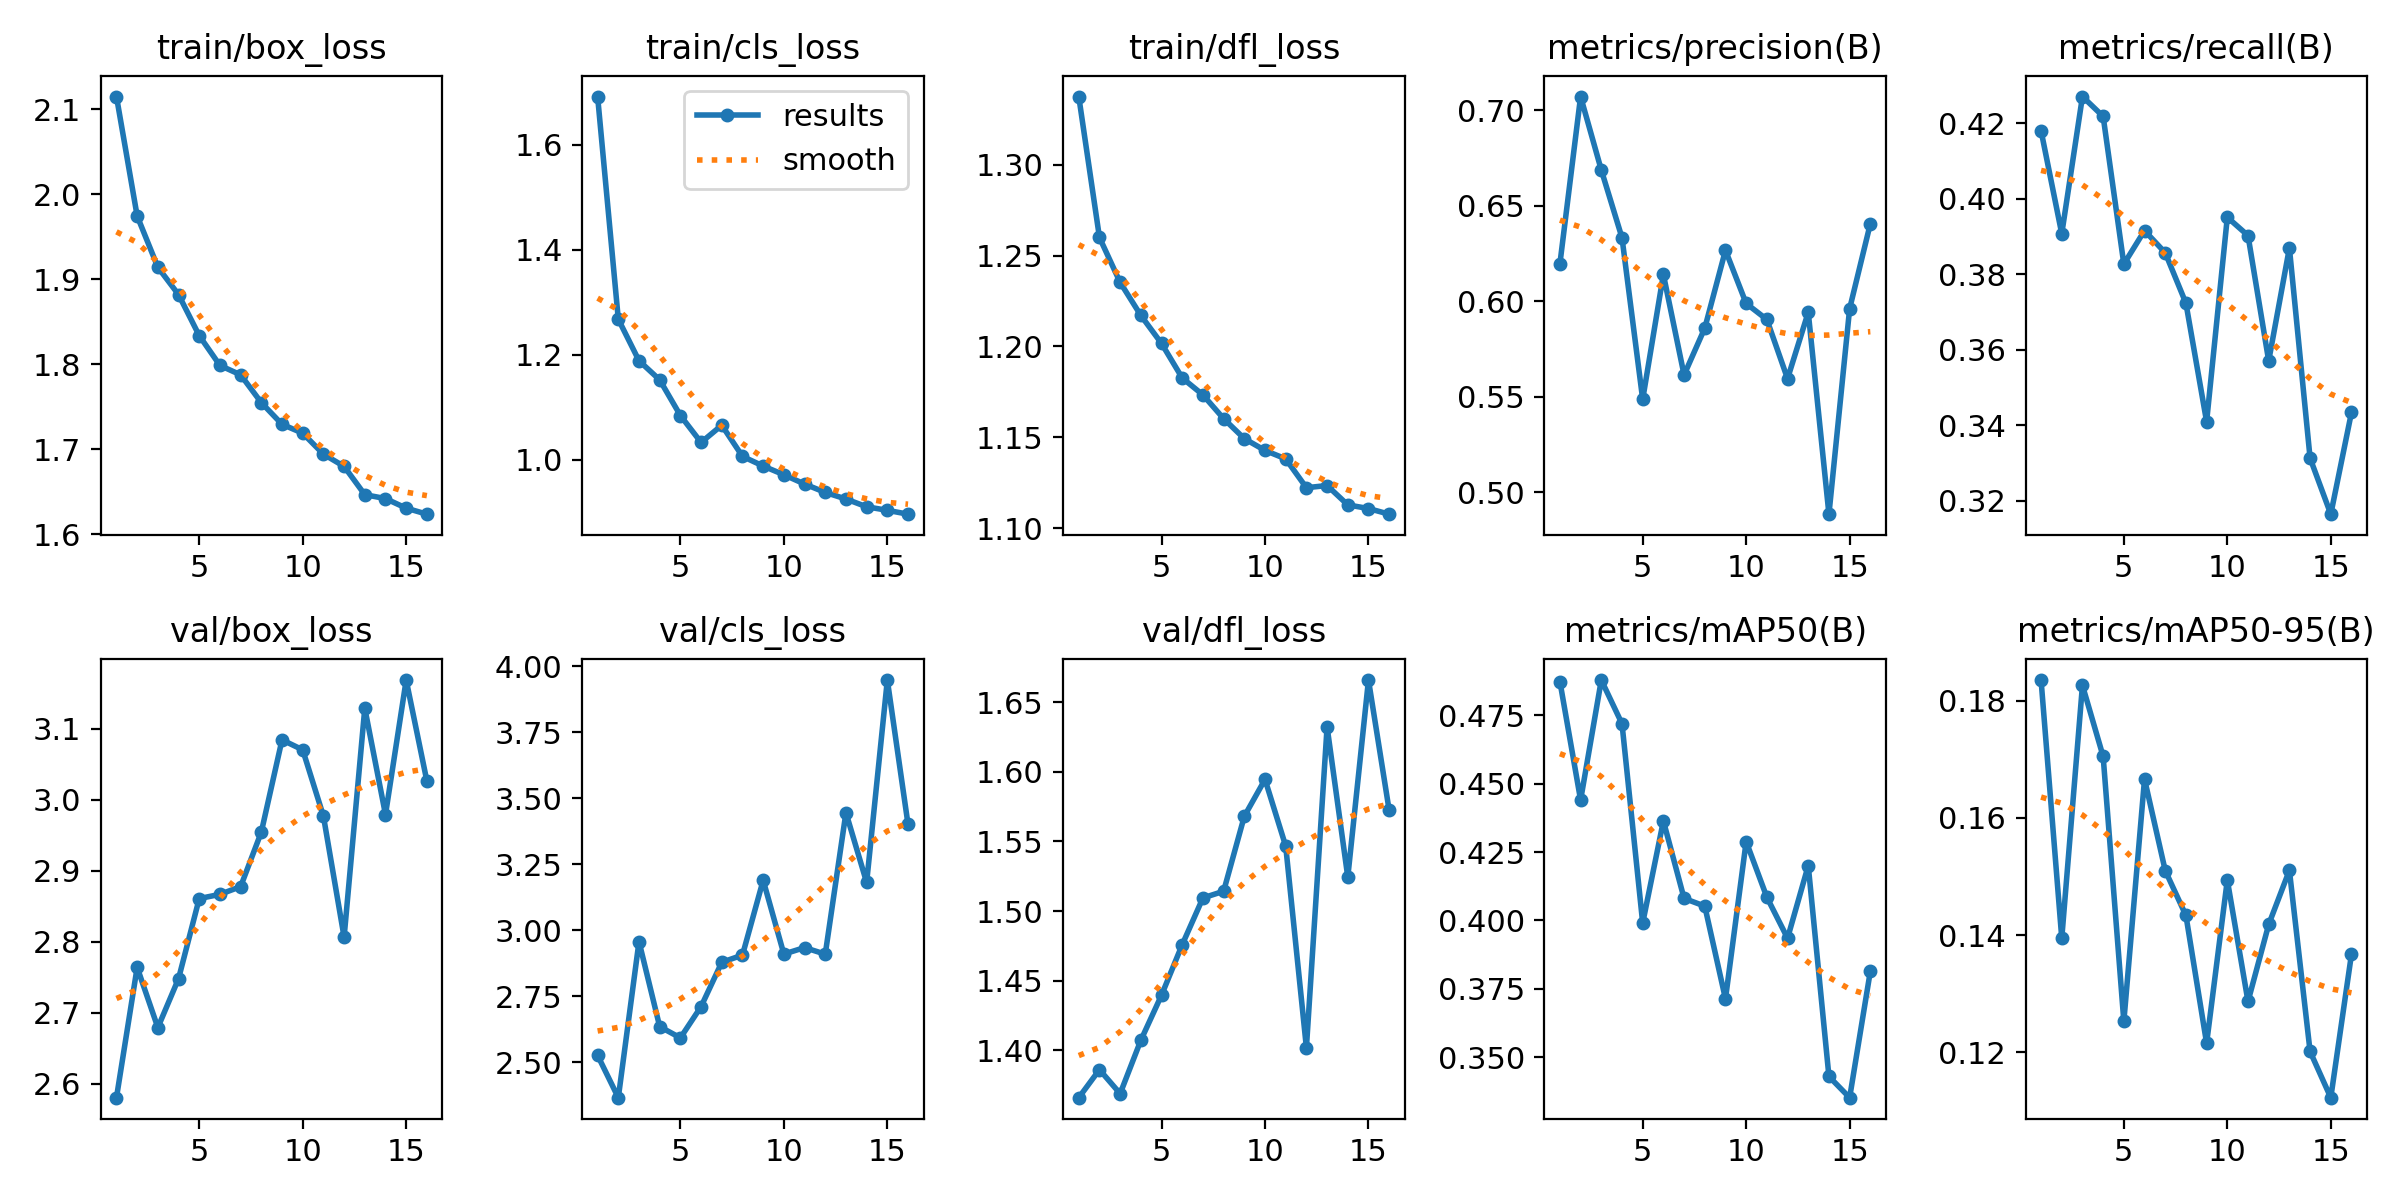
\includegraphics[width=\linewidth]{results.png}
  \caption{Training curves (loss and metrics) over 16 epochs.}
  \label{fig:curves}
\end{figure}

\begin{figure}[t]
  \centering
  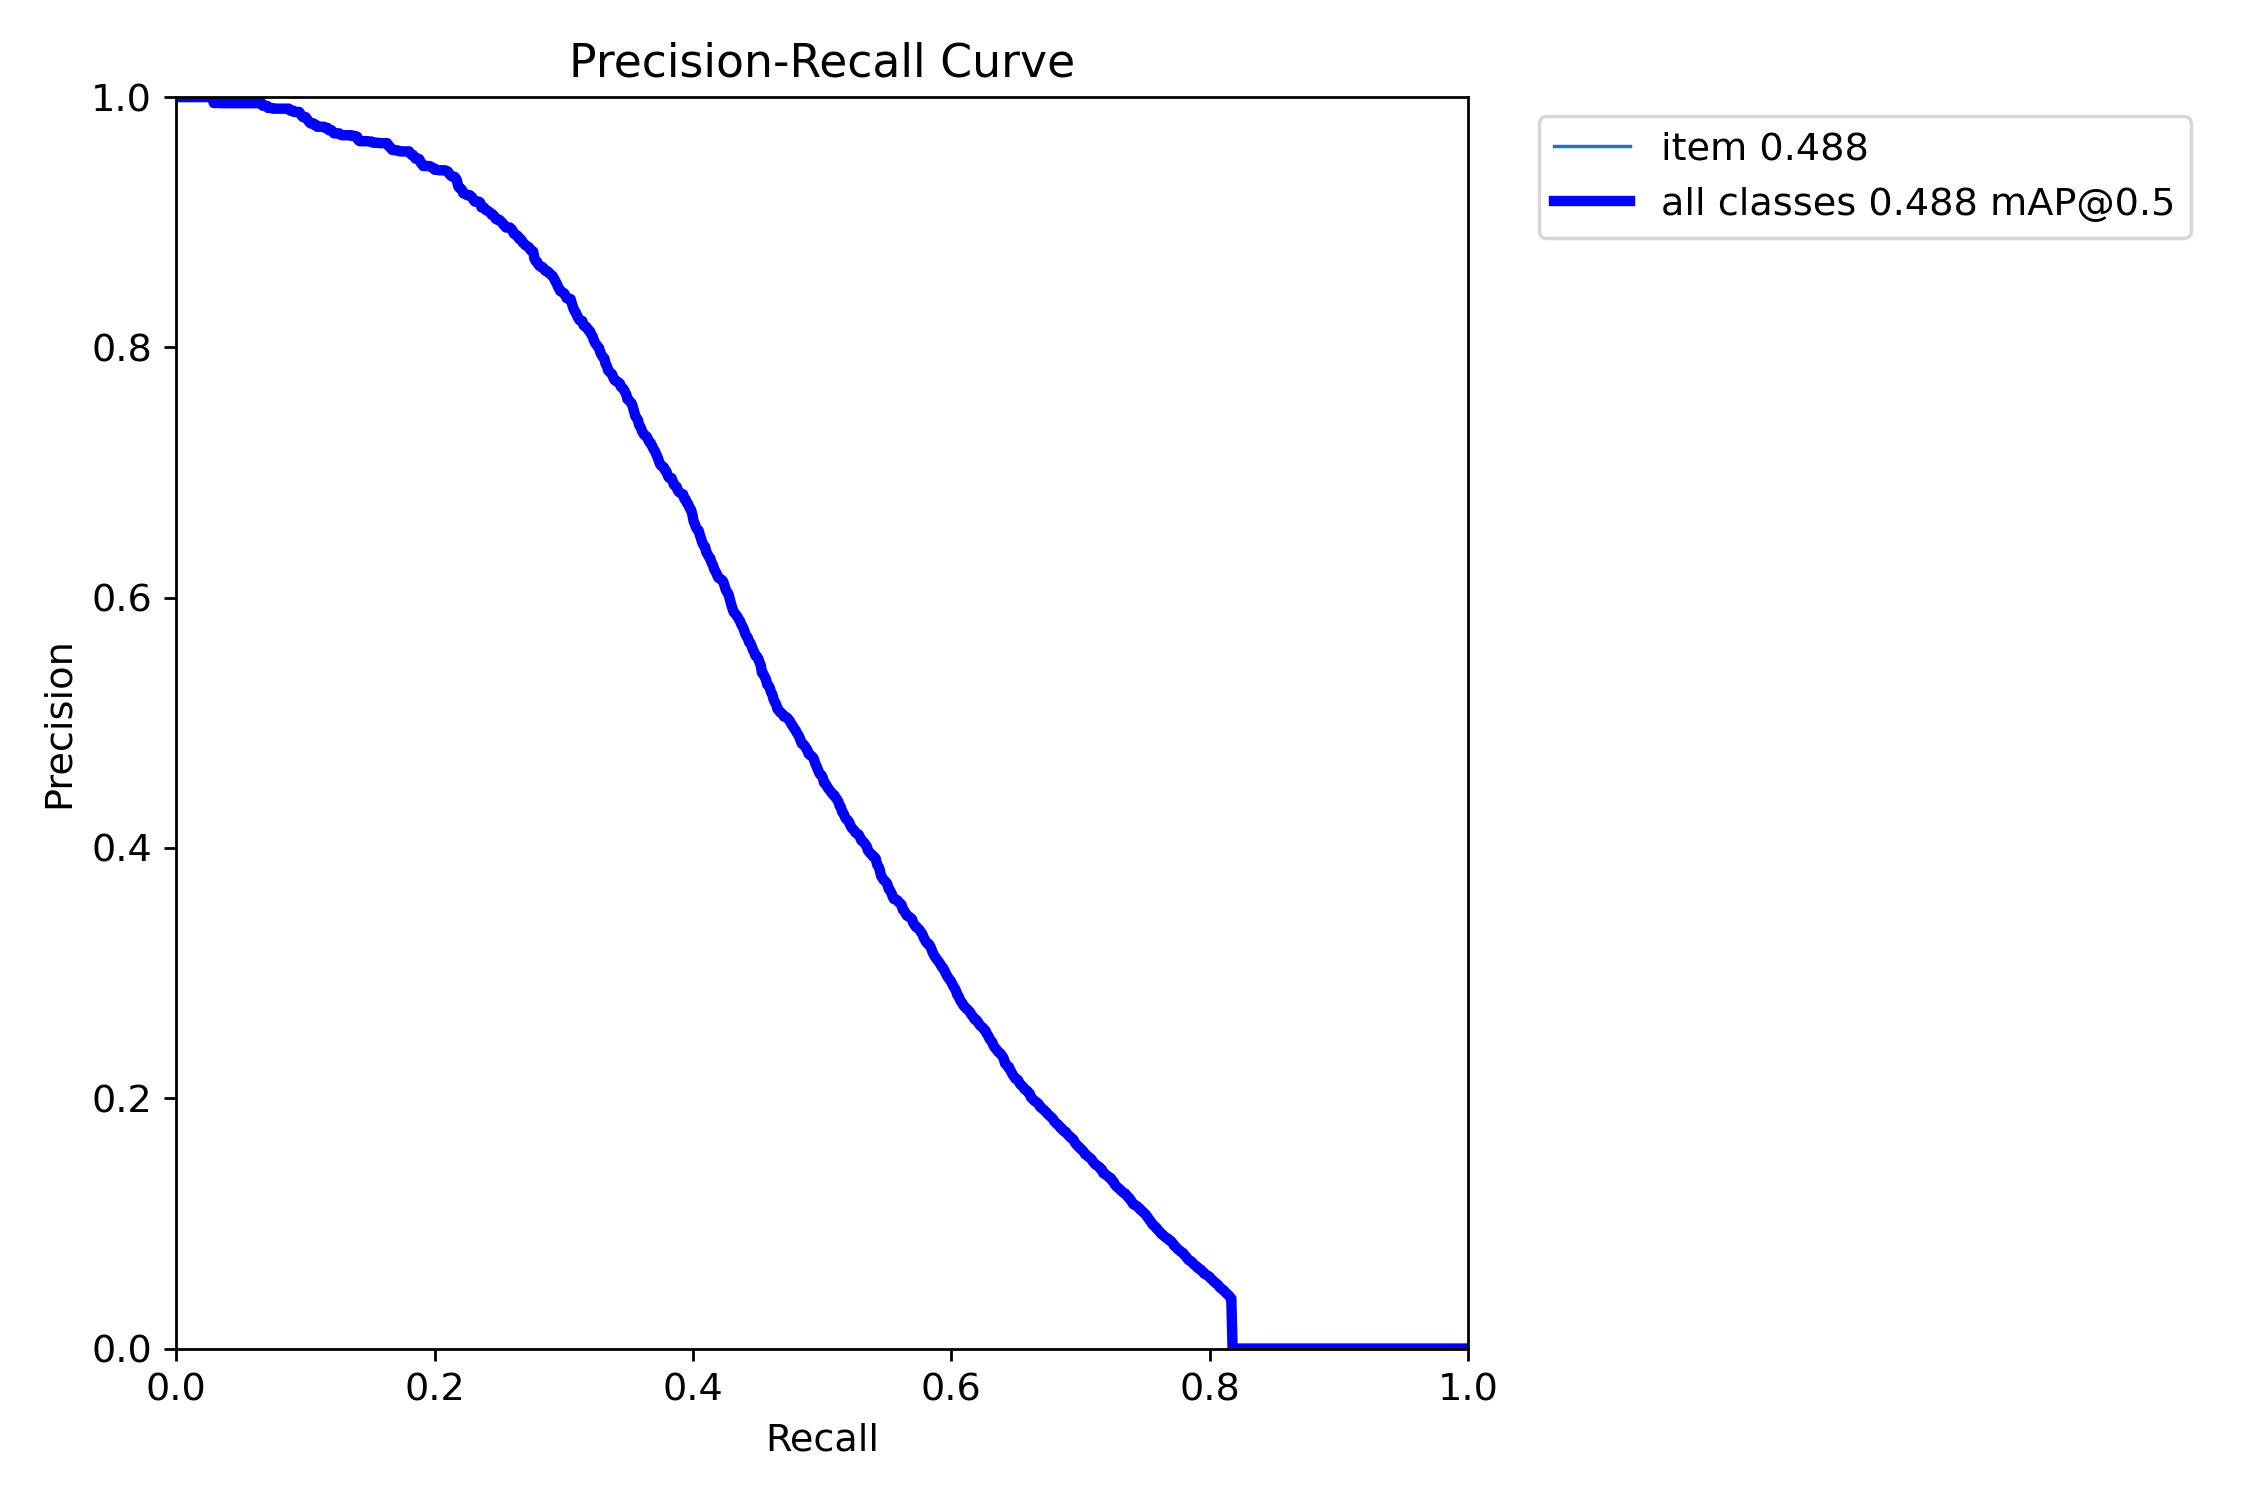
\includegraphics[width=\linewidth]{BoxPR_curve.png}
  \caption{Precision--recall curve (person class).}
  \label{fig:pr}
\end{figure}

\begin{figure}[t]
  \centering
  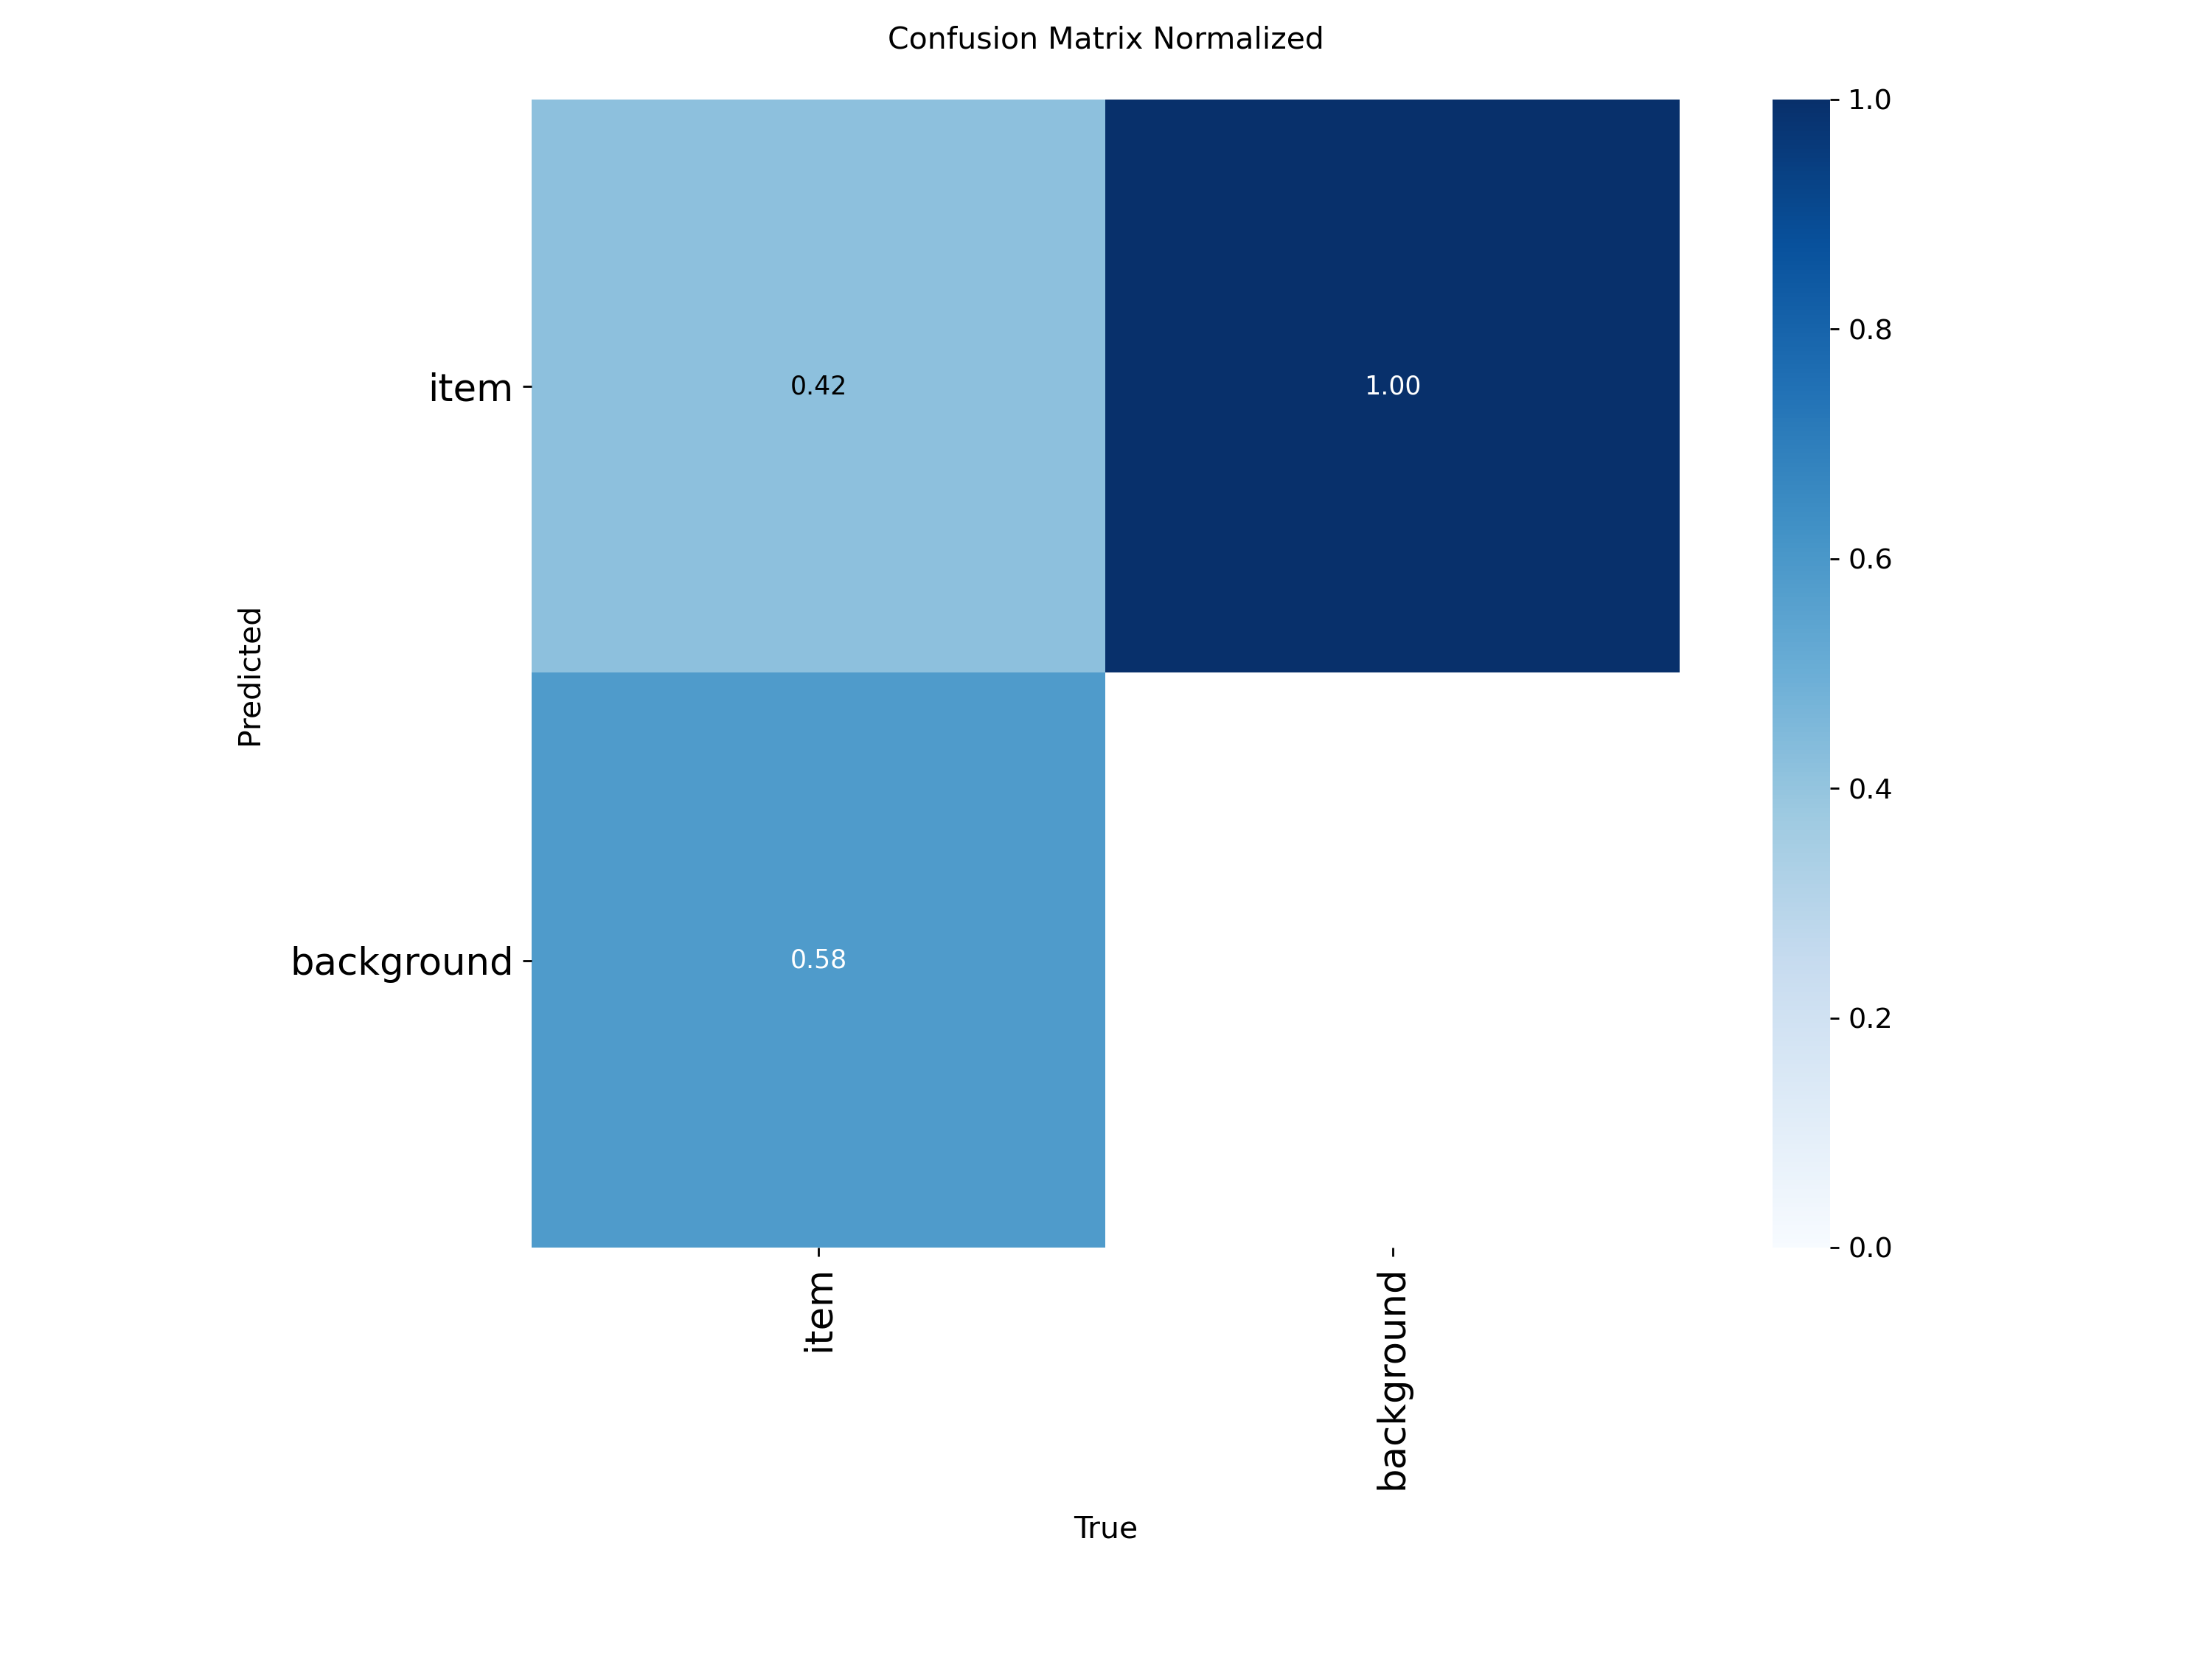
\includegraphics[width=0.48\linewidth]{confusion_matrix_normalized.png}
  \hfill
  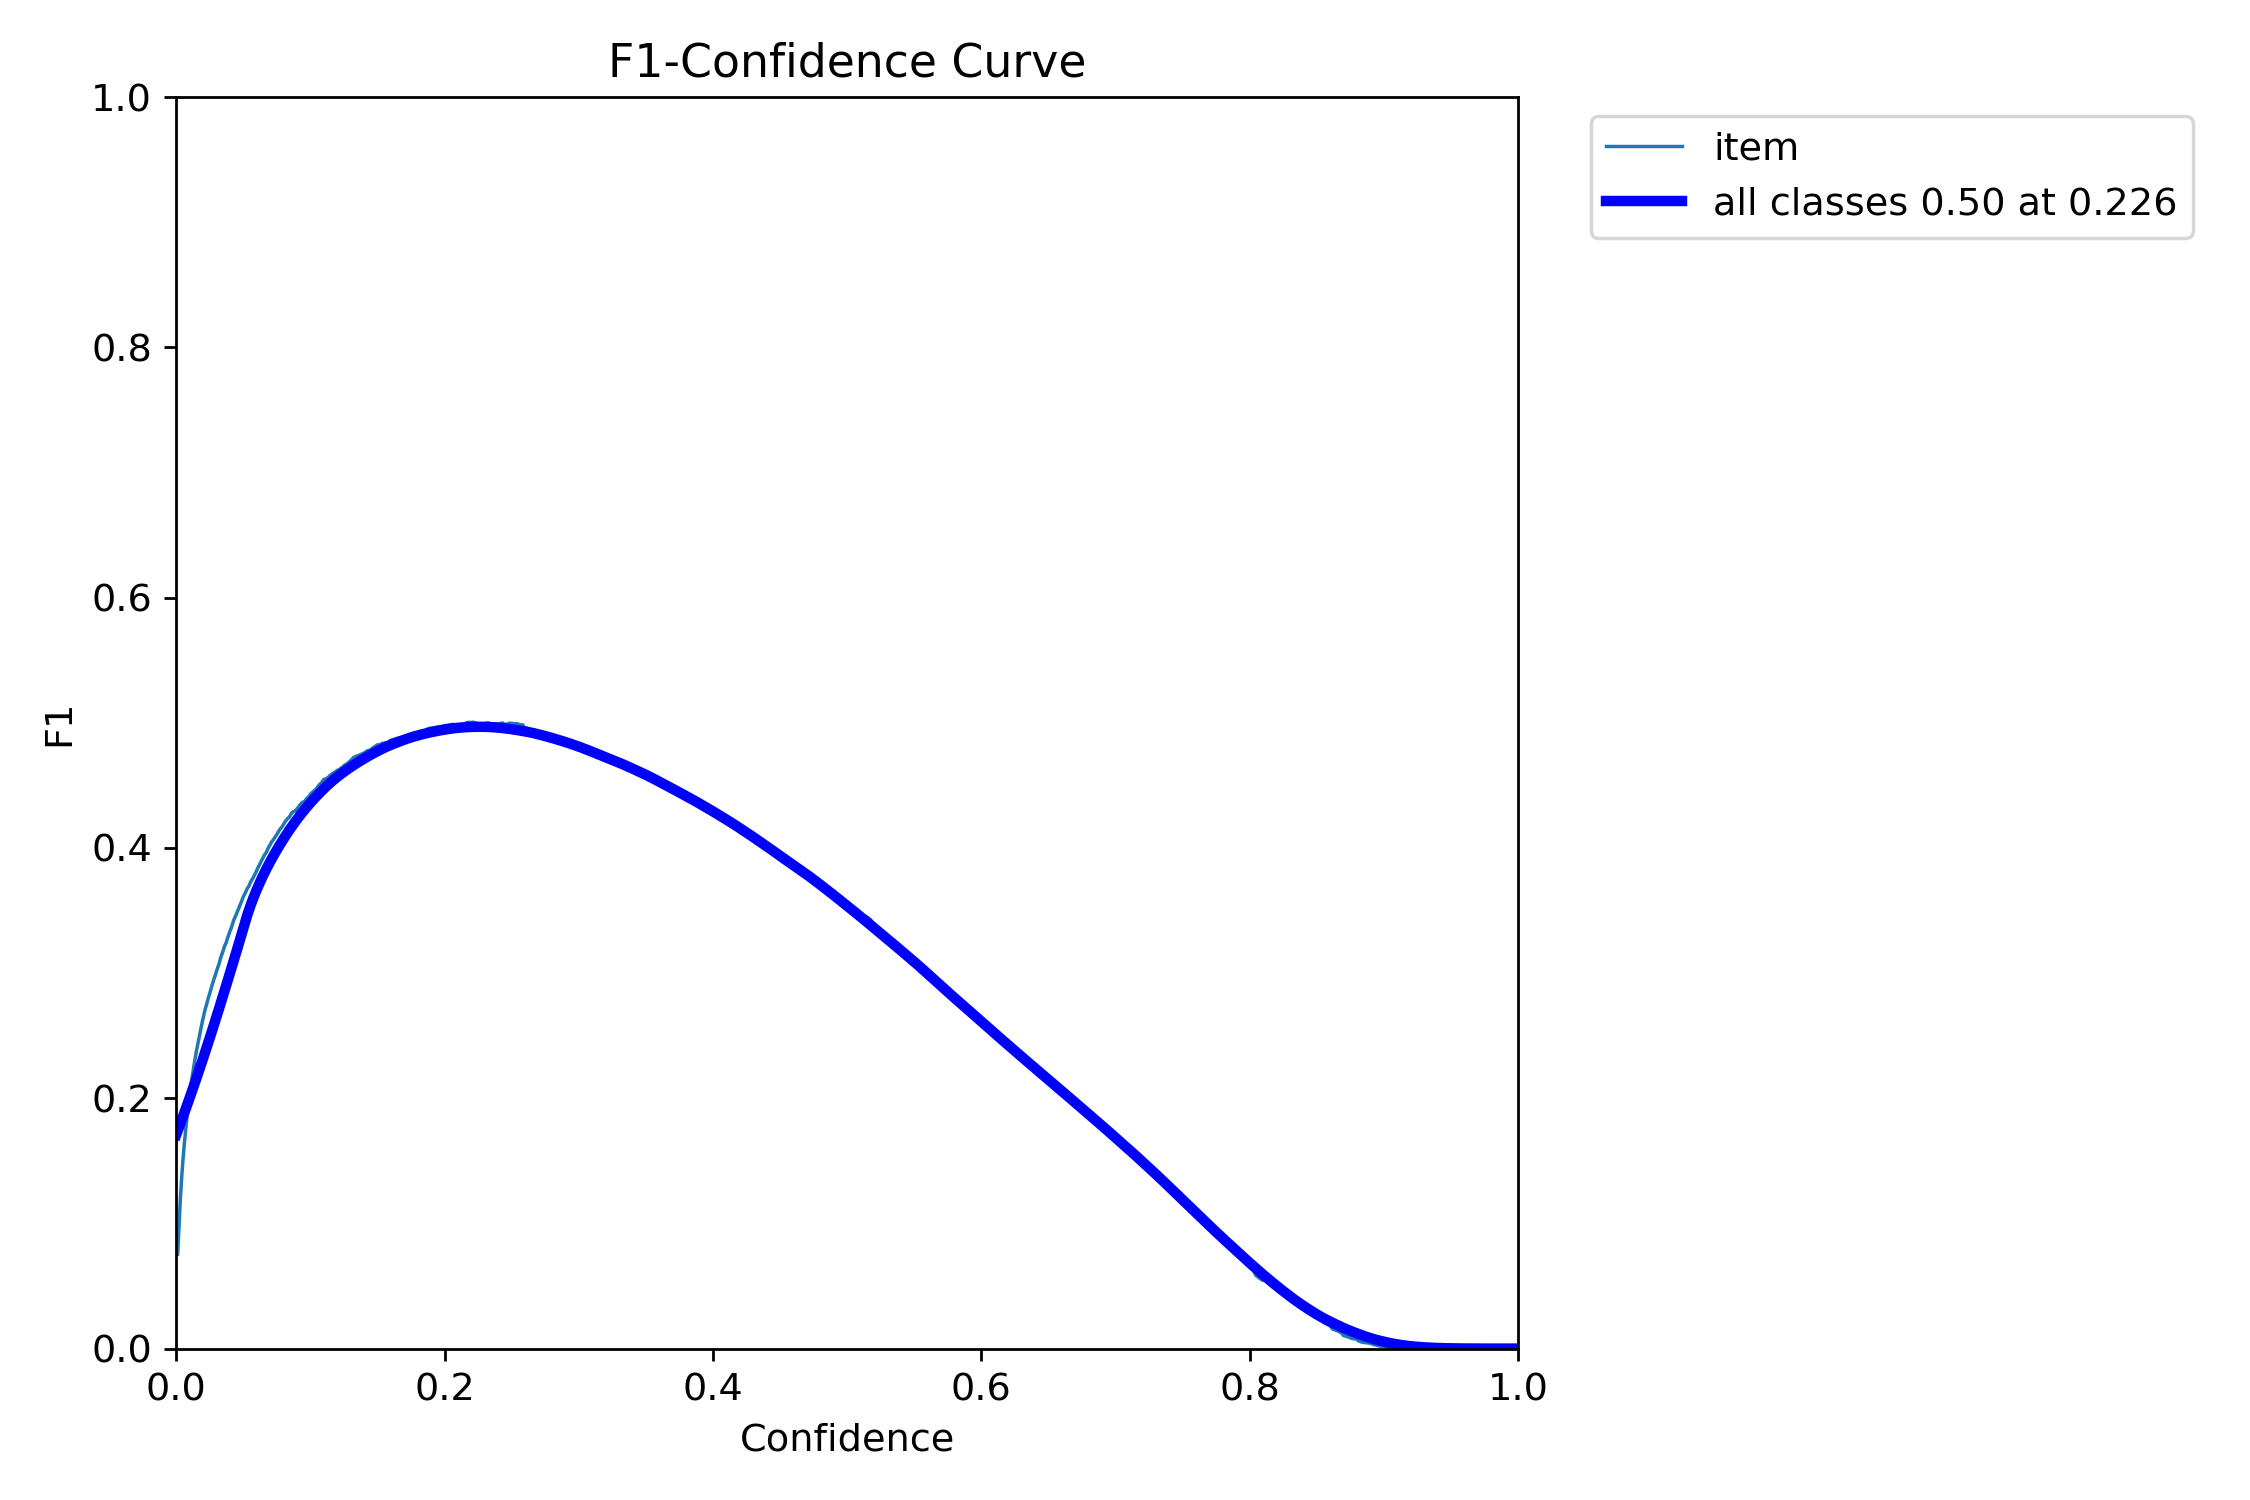
\includegraphics[width=0.48\linewidth]{BoxF1_curve.png}
  \caption{Normalized confusion matrix (left) and F1 curve (right).}
  \label{fig:cm_f1}
\end{figure}

\subsection{Qualitative Detection}
Figure~\ref{fig:qual} compares ground-truth labels and model predictions on a validation batch. Small pedestrians remain challenging at distance; high-resolution training improves but does not eliminate false negatives in dense regions.

\begin{figure}[t]
  \centering
  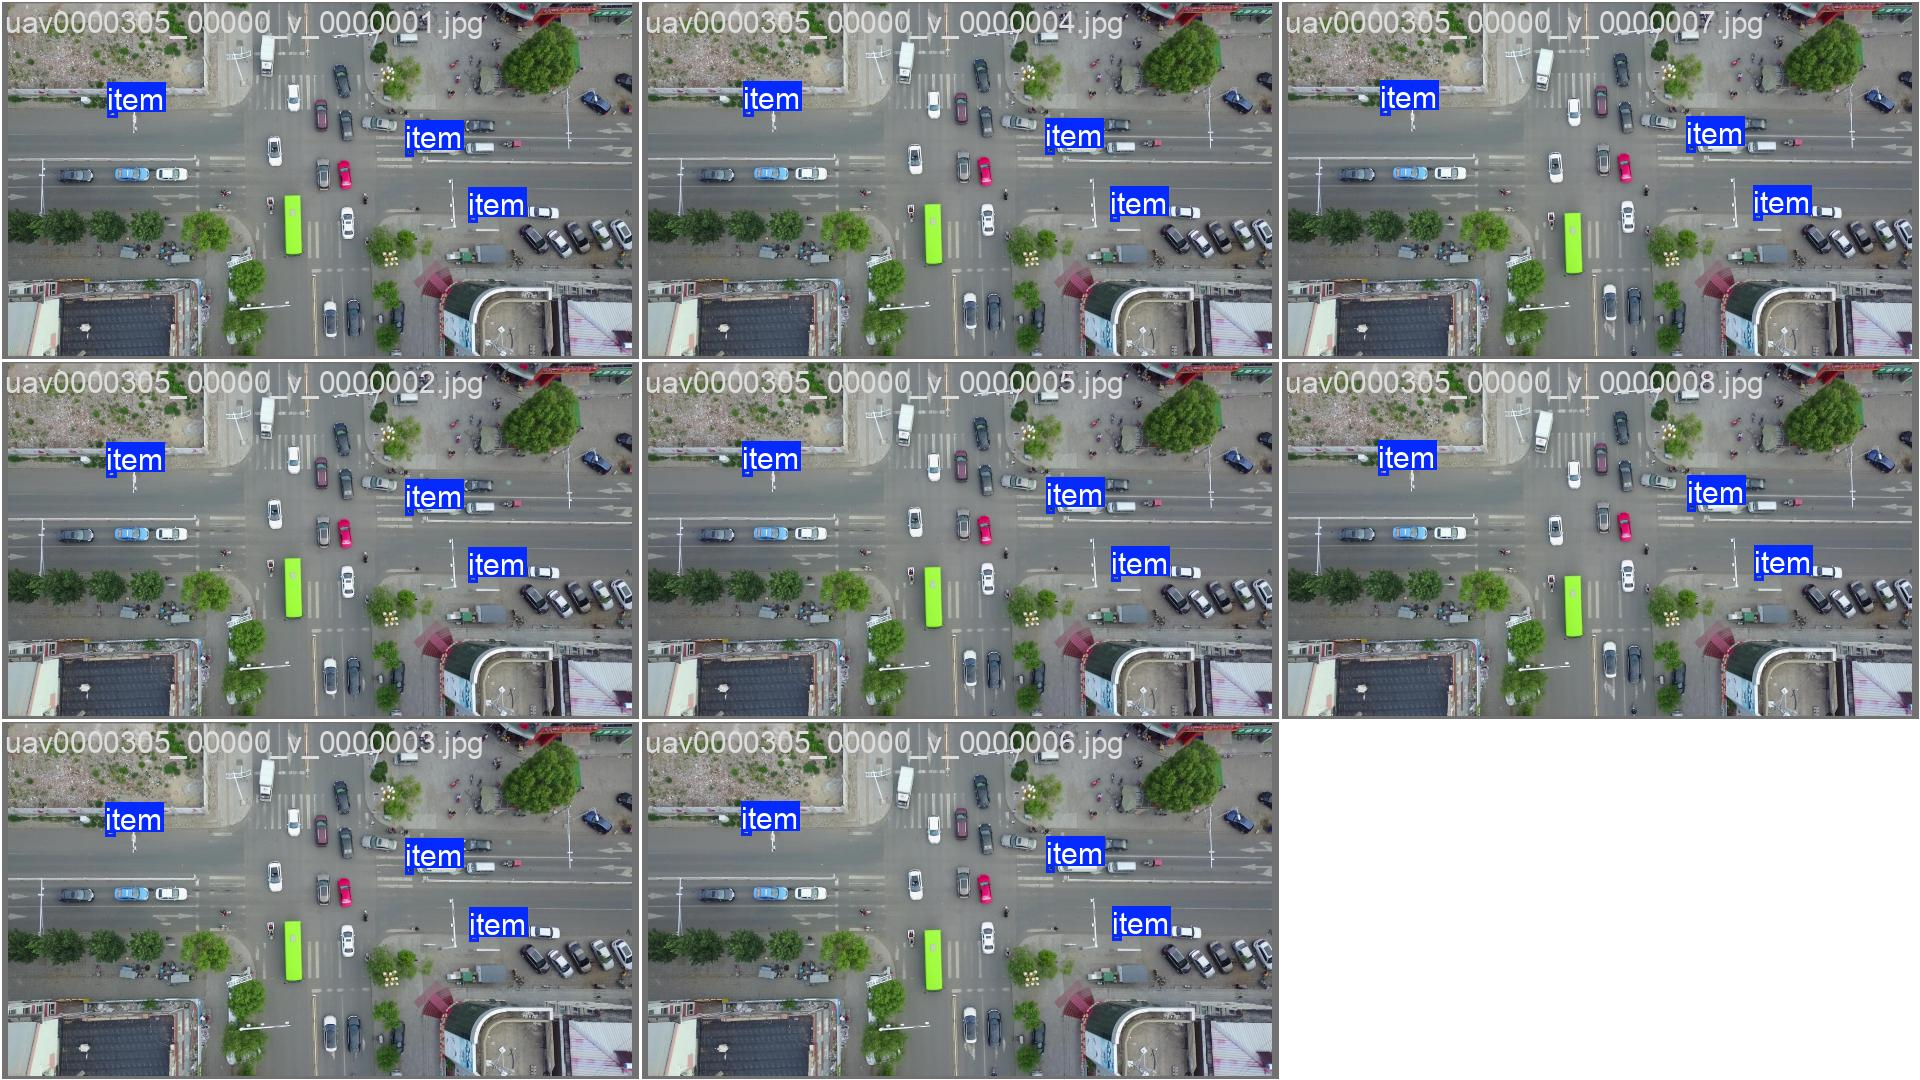
\includegraphics[width=\linewidth]{val_batch0_labels.jpg}
  \\[0.2em]
  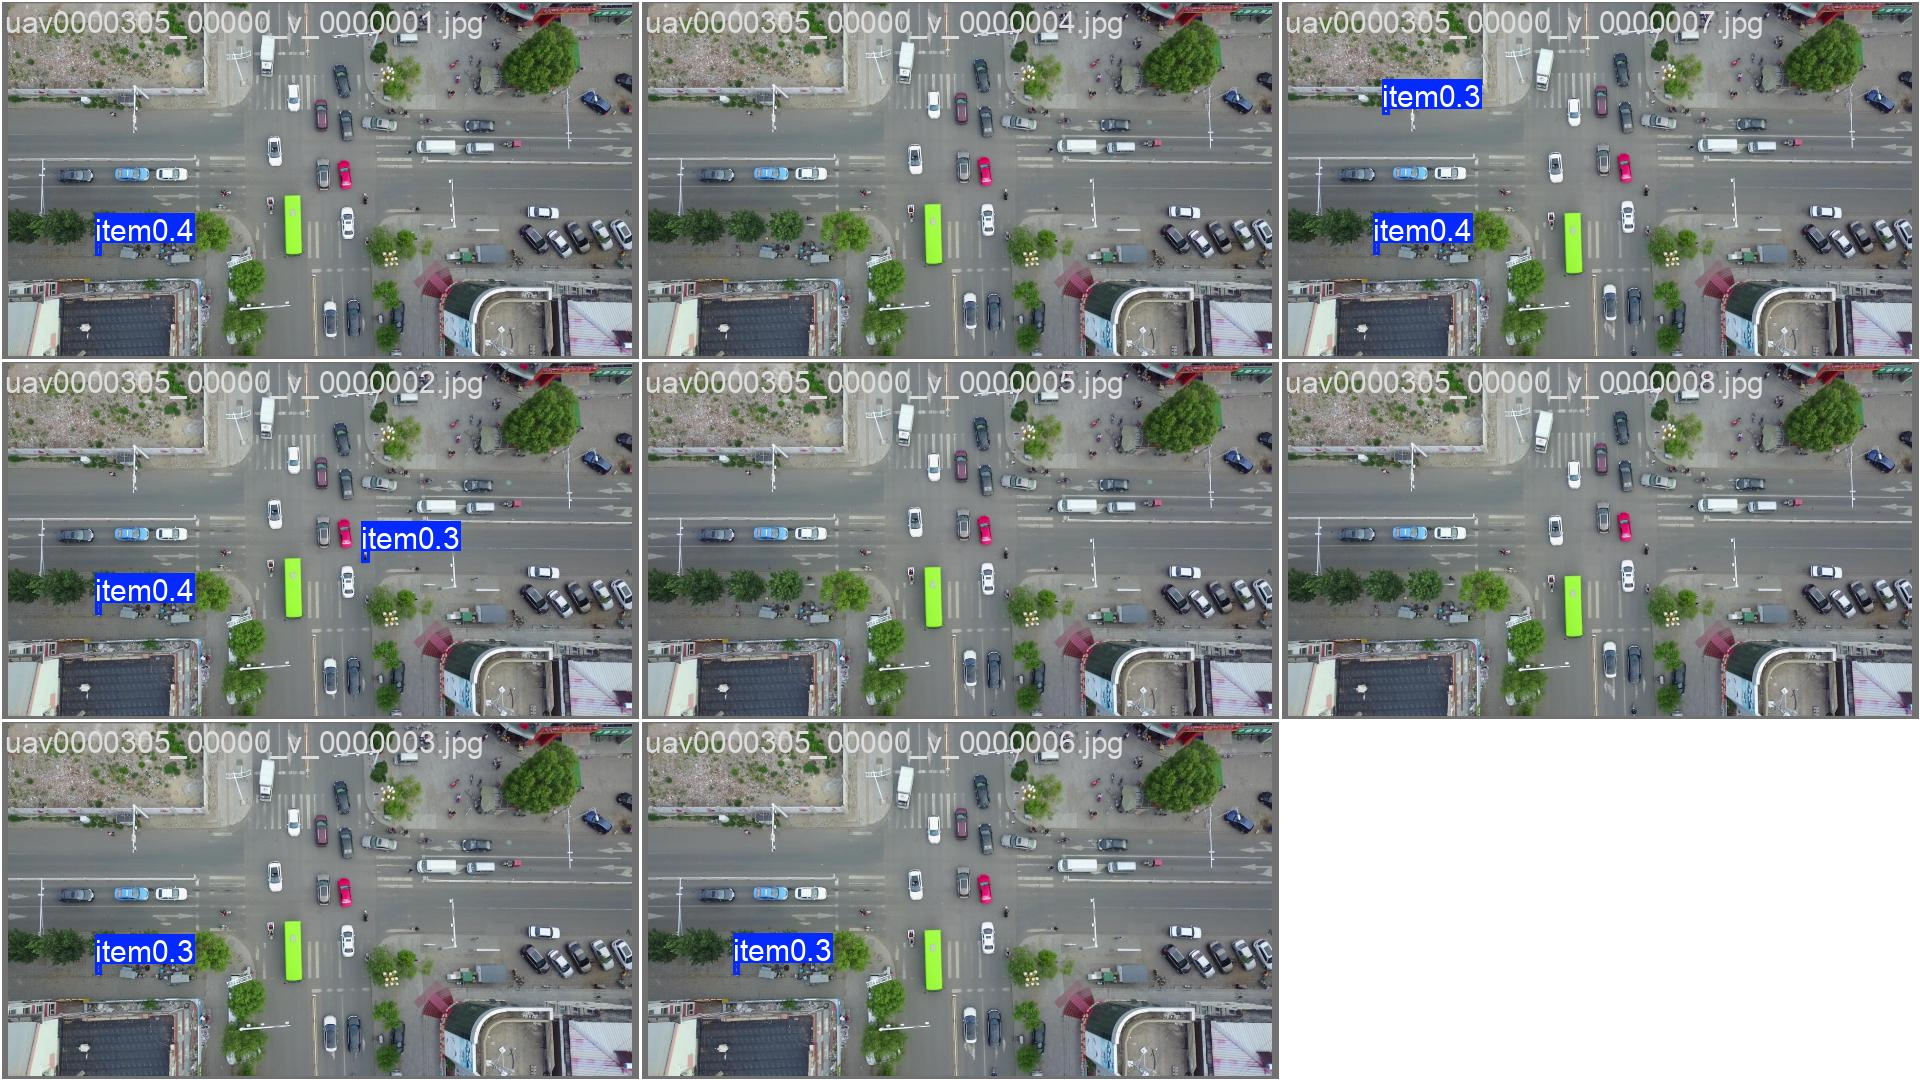
\includegraphics[width=\linewidth]{val_batch0_pred.jpg}
  \caption{Validation batch: labels (top) vs.\ predictions (bottom).}
  \label{fig:qual}
\end{figure}

\subsection{Dataset and Augmentation Statistics}
\begin{figure}[t]
  \centering
  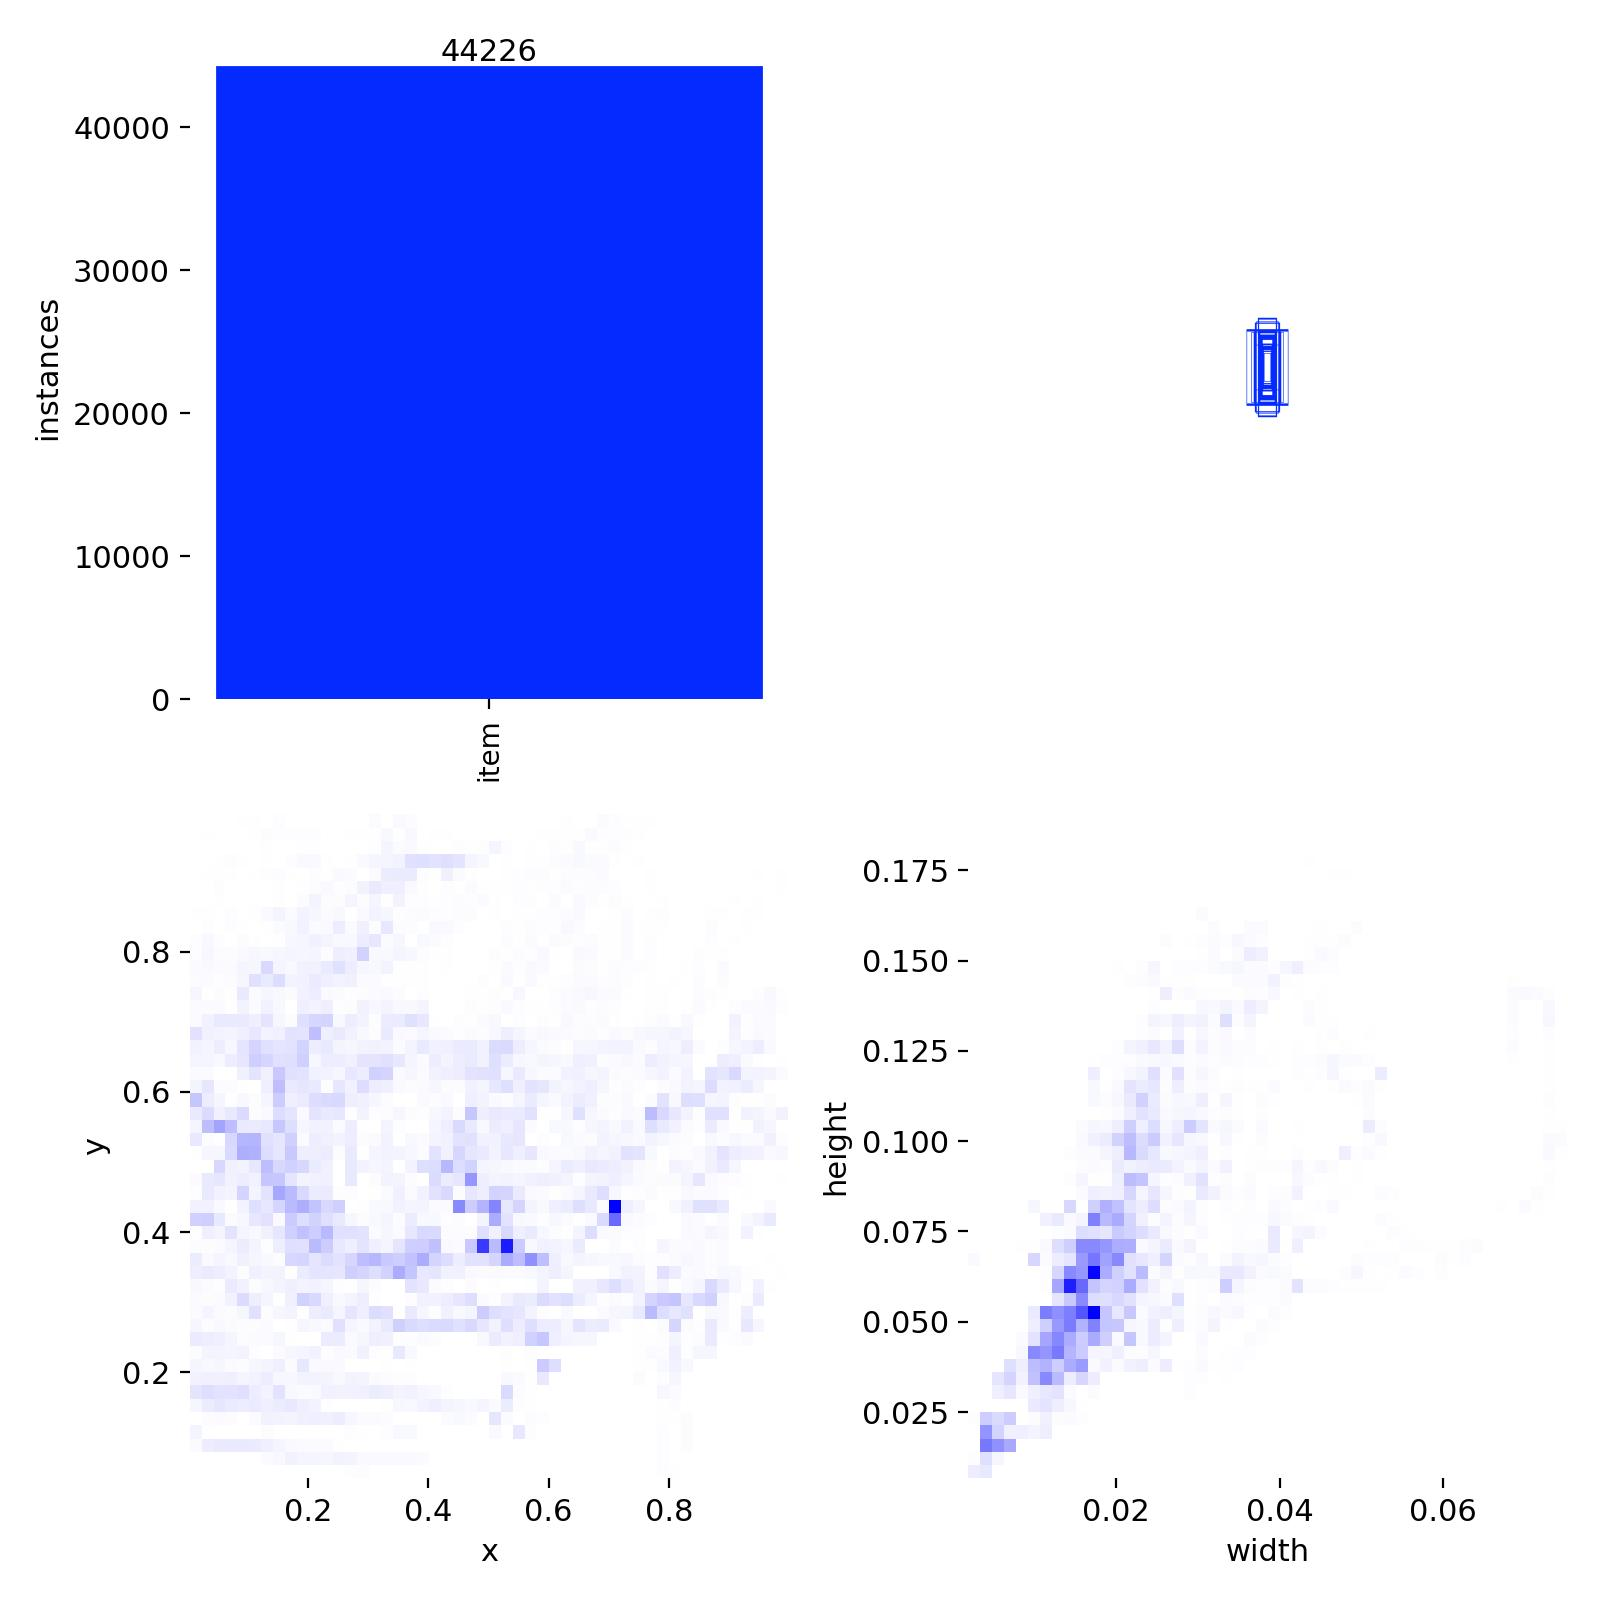
\includegraphics[width=\linewidth]{labels.jpg}
  \caption{Label distribution and spatial density after YOLO conversion.}
  \label{fig:labels}
\end{figure}

\begin{figure}[t]
  \centering
  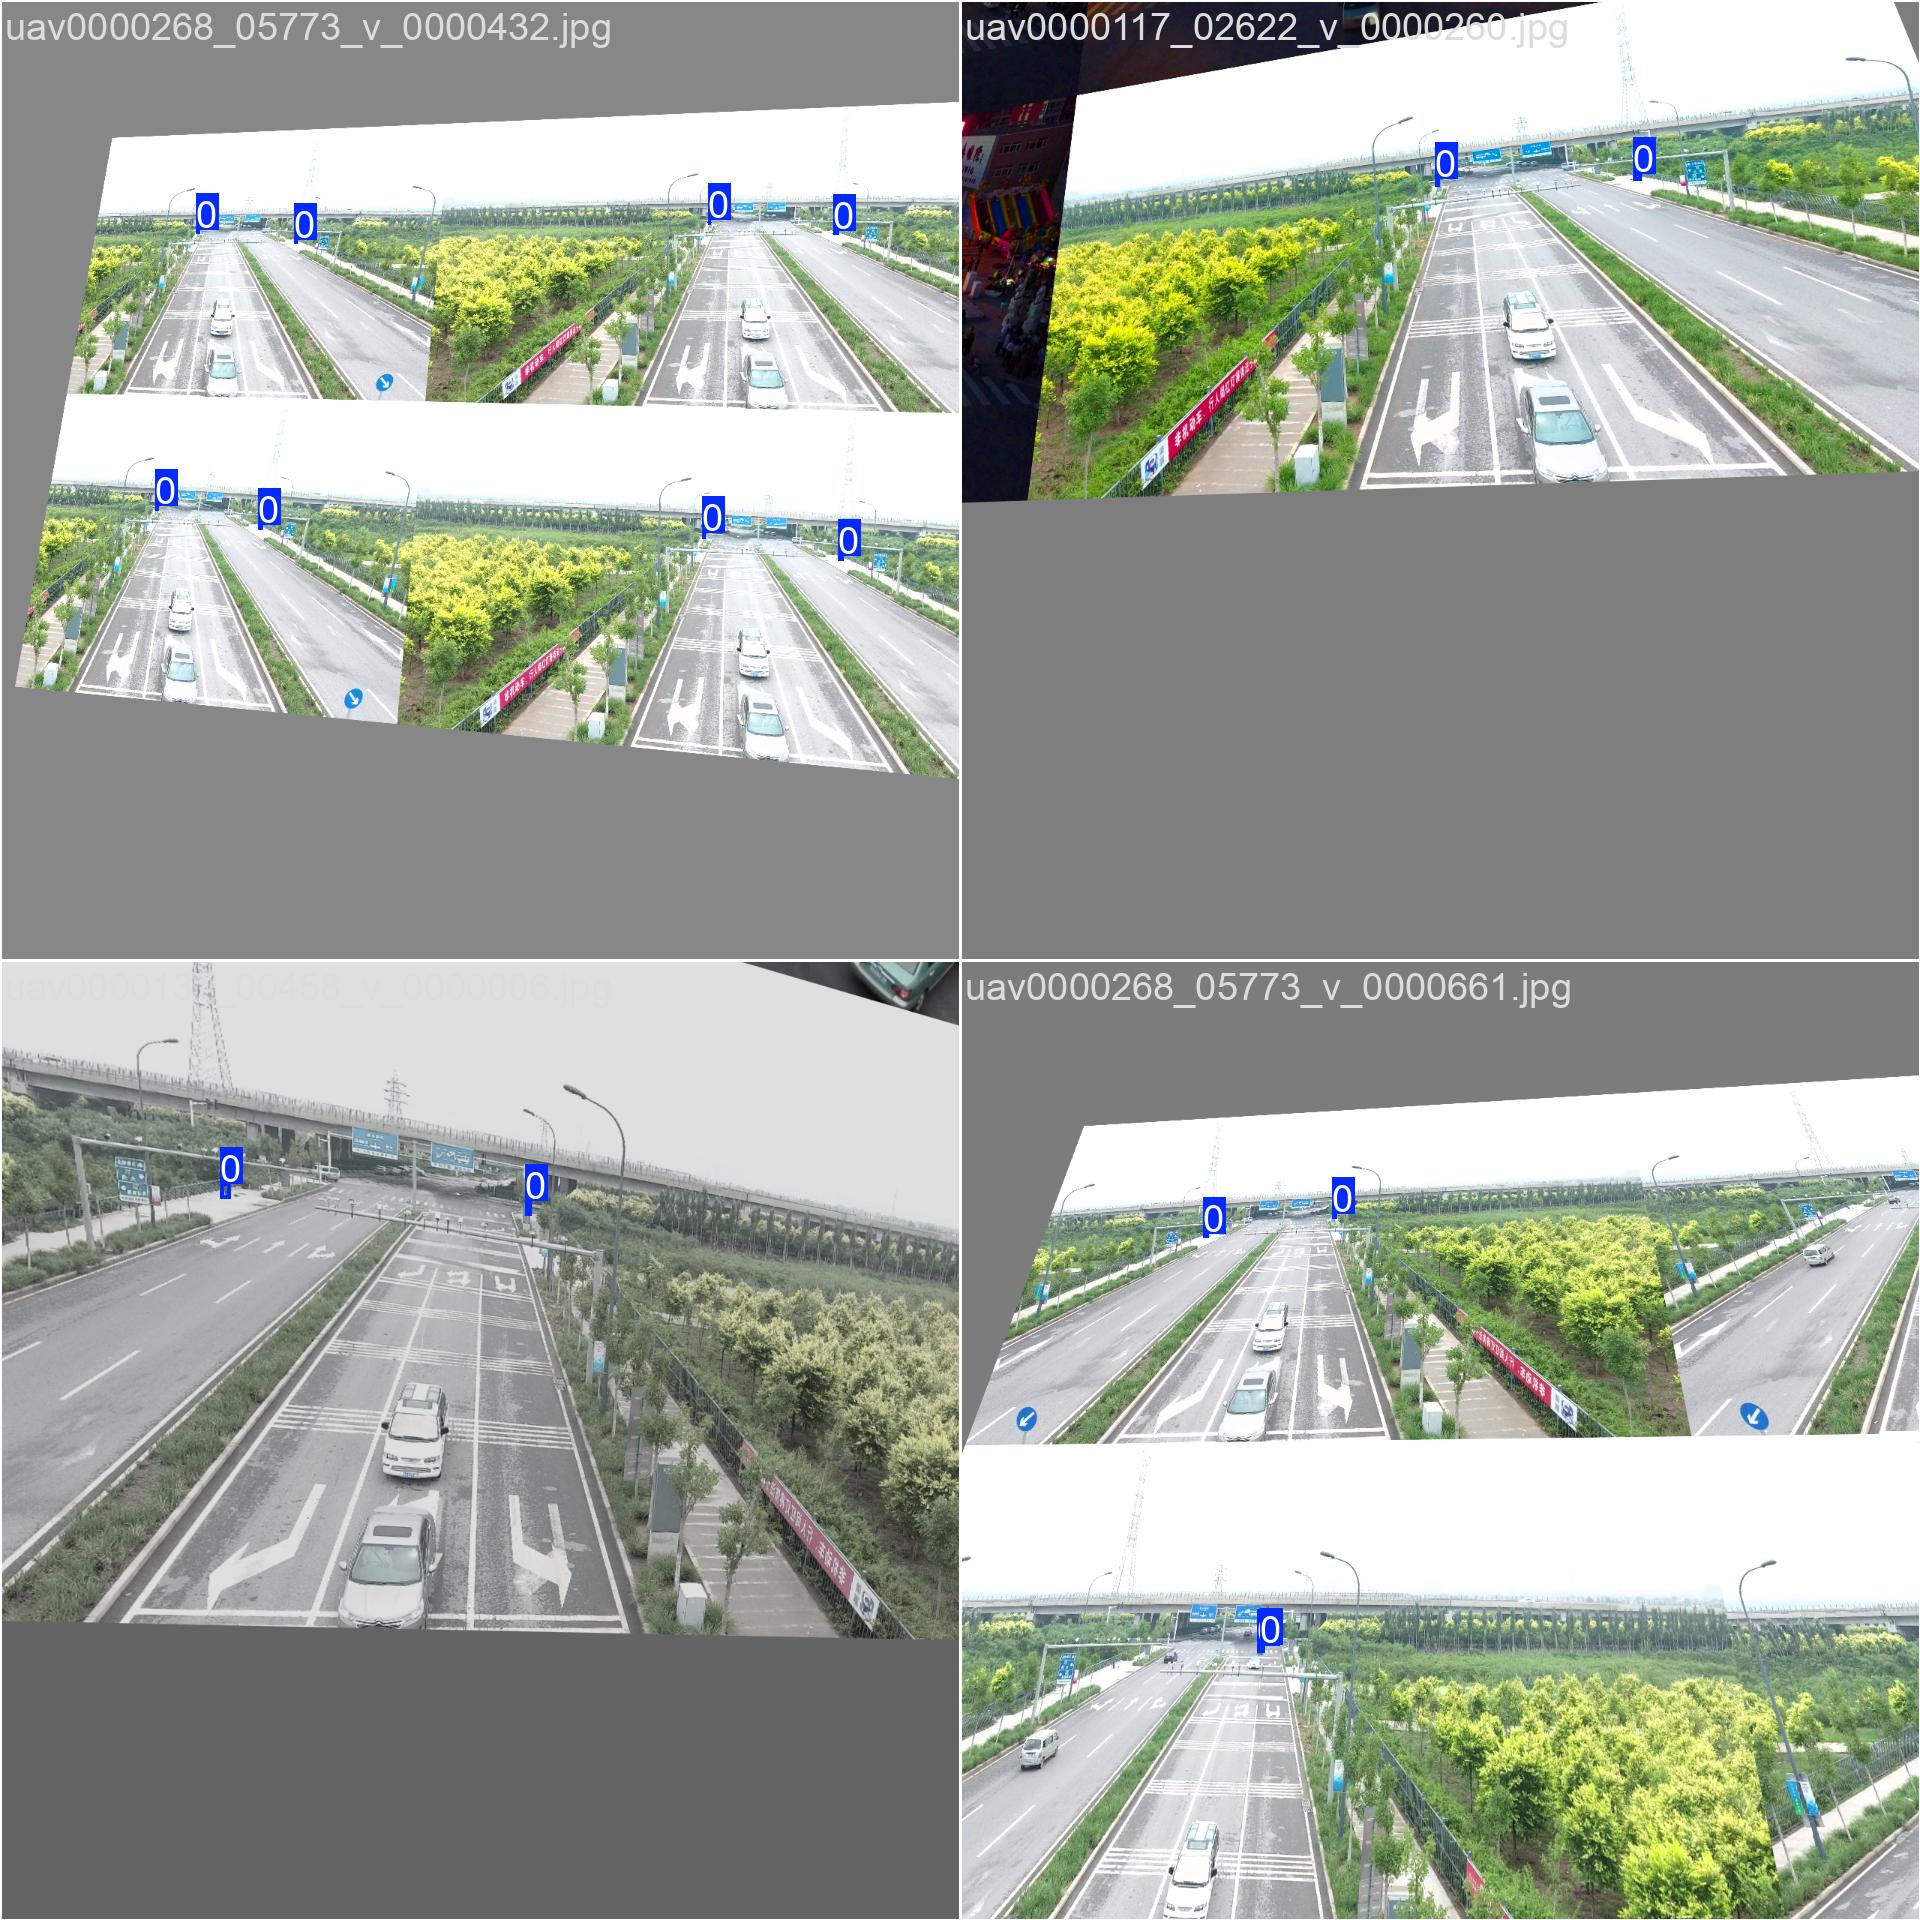
\includegraphics[width=\linewidth]{train_batch0.jpg}
  \caption{Training batch mosaic (epoch 1) showing augmented aerial crops.}
  \label{fig:mosaic}
\end{figure}

\subsection{Tracking and Demo Video}
We render sequence \texttt{uav0000086\_00000\_v} (464 frames) with bounding boxes, \texttt{ID:k} labels, confidence scores, and 25-frame trajectory tails. Output: \texttt{outputs/videos/demo\_uav0000086.mp4} (61\,MB).

\textbf{ID switching.} Residual switches occur during occlusion and pedestrian crossing; mitigations include extended \texttt{track\_buffer}, low detection threshold, and Kalman smoothing. Global motion compensation (BoT-SORT GMC) is noted as a future upgrade if CPU budget allows.

\subsection{Latency and Throughput}
Table~\ref{tab:fps} summarizes end-to-end measurements (frame read $\rightarrow$ detect $\rightarrow$ track; demo row includes H.264 encode).

\begin{table}[h]
\centering
\caption{Pipeline throughput (RTX A4000 \#0, FP16, ByteTrack).}
\label{tab:fps}
\small
\begin{tabular}{lccc}
\toprule
Mode & Frames & ms/frame & FPS \\
\midrule
Benchmark & 200 & 5.24 & \textbf{190.7} \\
Demo render & 464 & 6.27 & 159.4 \\
\bottomrule
\end{tabular}
\end{table}

\textbf{Model size:} \texttt{best.pt} = 6.1\,MB (total deployable artifacts $\ll$ 300\,MB).

\subsection{Engineering Trade-off Analysis}
\begin{itemize}[leftmargin=*, nosep]
    \item \textbf{1280 train / 960 infer:} preserves small-target learning while meeting real-time goals on datacenter GPUs; Jetson should use 640--736.
    \item \textbf{ByteTrack vs.\ DeepSORT:} eliminates ReID ($\sim$50--100\,MB + embedding latency) at cost of more ID switches in appearance-similar crowds.
    \item \textbf{Tiled inference:} improves recall on micro-objects; omitted in FPS table due to $>3\times$ compute.
\end{itemize}

\section{Edge Deployment}
\label{sec:edge}
For NVIDIA Jetson (Orin NX / AGX):
\begin{enumerate}[leftmargin=*, nosep]
    \item Export \texttt{best.pt} $\rightarrow$ ONNX $\rightarrow$ TensorRT FP16 engine.
    \item Run inference at 640--736\,px; keep ByteTrack on CPU.
    \item Disable tiling; optional async GStreamer capture thread.
    \item Expect 25--60\,FPS depending on module and power mode (not re-benchmarked on silicon in this submission).
\end{enumerate}

\section{Conclusion}
We described a lightweight, VisDrone-adapted person detection and tracking pipeline combining YOLOv8n fine-tuning and ByteTrack. The system meets the model size constraint, documents quantitative and visual results, and achieves $>$150\,FPS on RTX A4000 hardware at 960\,px inference. Future work includes MOT train split fine-tuning, BoT-SORT GMC, and on-device Jetson profiling.

\section*{Reproducibility}
Code: \url{https://github.com/rishi02102017/The-Aerial-Guardian-Challenge}. Dataset: VisDrone2019-MOT-val (user download). Commands in repository \texttt{README.md}.

{\small
\bibliographystyle{ieee}
\begin{thebibliography}{9}
\bibitem{visdrone}
P.~Zhu et al., ``VisDrone-DET2019: The Vision Meets Drone Object Detection in Image Challenge Results,'' ICPR Workshops, 2019.
\bibitem{yolo}
J.~Redmon et al., ``You Only Look Once: Unified, Real-Time Object Detection,'' CVPR, 2016. Ultralytics YOLOv8, 2023.
\bibitem{bytetrack}
Y.~Zhang et al., ``ByteTrack: Multi-Object Tracking by Associating Every Detection Box,'' ECCV, 2022.
\end{thebibliography}
}

\end{document}
